\chapter{Requirement Analysis and Specification}

The MLUD will offer the following functionalities:
\begin{itemize}
    \item User registration and book detail submission via an online form.
    \item Facilitating the physical handover of books, including verification and labeling.
    \item Streamlining the sales process with a digital interface for managing transactions.
    \item Tracking unsold books and managing financial settlements for sellers.
    \item Generating aggregated statistical reports to monitor performance and user satisfaction.
\end{itemize}

\section{Hardware Interfaces}
The system will be accessible through a web interface. The PR will have the option to use both a computer and a mobile device to access the system, so the interface must be responsive and usable on both platforms.

The OP will use a computer to access the system, so the interface must be optimized for computer use.

\section{Use Cases}

The use cases are illustrated in the diagram in Figure \ref{fig:use_cases}.

\begin{figure}[h]
    \centering
    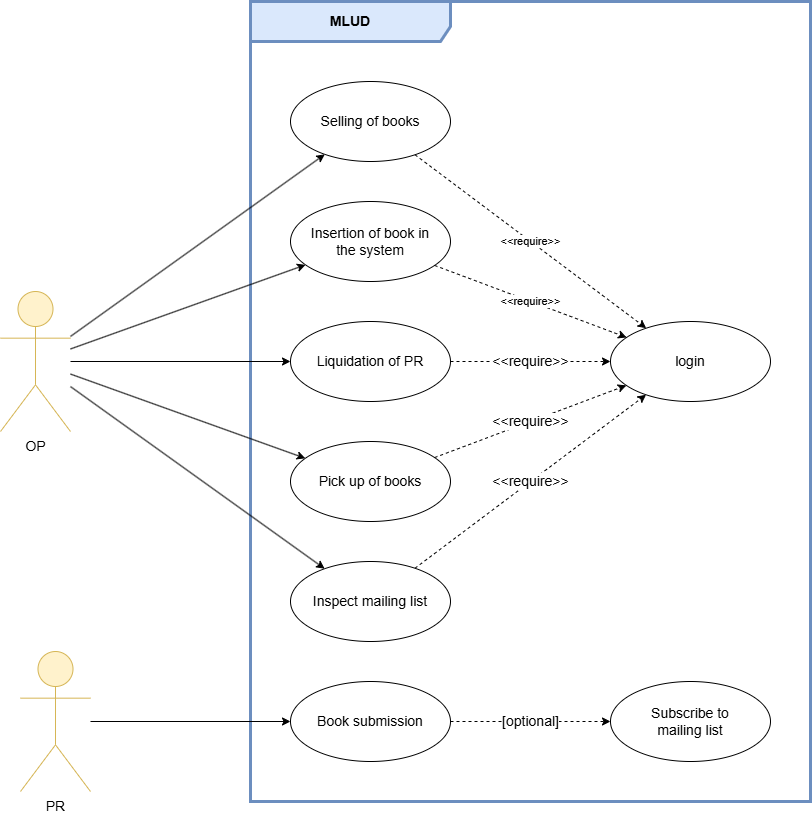
\includegraphics[width=.75\textwidth]{assets/use_cases_diagram.png}
    \caption{Use cases diagram}
    \label{fig:use_cases}
\end{figure}

\subsection{Use Case 1: Book submission}

\begin{enumerate}
    \item The PR accesses the system.
    \item The PR fills out the form, providing:
          \begin{itemize}
              \item Personal information (name, surname, email, phone number).
              \item Information for an arbitrary number of books (ISBN, title, author, edition, price, condition).
              \item Acceptance of the terms and conditions.
              \item Preference for subscription to the mailing list.
          \end{itemize}
          When entering the ISBN, the system will suggest the book's information if it is already in the system.
    \item The PR submits the form, it is redirected to a confirmation page and receives a confirmation email.
\end{enumerate}


\subsection{Use Case 2: Book delivery}

\begin{enumerate}
    \item The PR goes to Lokalino with the books.
    \item The OP accesses the protected area of the system.
    \item The OP searches for the record of the PR in the system.
    \item The OP verifies the correspondence between the books and the records, eventually updating the records or adding comments
    \item If all is correct, the OP labels the books to identify the corresponding PR
    \item The OP mark the correct delivery of the books in the system
\end{enumerate}

\subsection{Use Case 3: Book sale}

\begin{enumerate}
    \item The OP accesses the protected area of the system.
    \item The BY selects the books they want to buy.
    \item For each book, the OP searches for the record in the system and adds the book to the cart.
    \item At the end of the selection, the OP confirms the purchase and collects the payment. The books are marked as sold in the system.
\end{enumerate}

\subsection{Use Case 4: Liquidation and return of unsold books}

\begin{enumerate}
    \item The OP accesses the protected area of the system.
    \item The OP searches for the record of the PR in the system.
    \item The system shows the list of books unsold and the total amount due to the PR.
    \item The PR collects the money and the unsold books.
    \item The OP marks the books as returned in the system.
\end{enumerate}

\section{Special Requirements}

In order to facilitate the filling of the form by the PR, the system will provide a search function that will suggest the book's information when the ISBN is entered. In order to generate this suggestion, the system will also allow the OP to manually enter the book's information, possibly before the beginning of the event.

The system will keep the data of the PRs and the books for 1 year after the event, and after that, it will be deleted. The only data that will be kept indefinitely is the list of persons who have subscribed to the mailing list.

\section{Assumptions}
\label{sec:assumptions}

A couple of assumptions have been made in the design of the system:

\begin{itemize}
    \item Even if in the implementation every PR will be identified by a unique ID, the system will check the uniqueness of the email address; this comes into play when a PR submits the form: if the email address is already in the system and the PR fills out the form again, the system will not create a new record and will work as if the same PR is inserting more books.
    \item Same thing for the ISBN: if the ISBN is already in the system, the system will suggest the book's information, and the PR will not have to fill out the form for that book. If the PR wants to insert different informations for a book that is already in the system (for example, a different price, or a different author), the system will discard the data inputted by the PR and will use the data already in the system.
\end{itemize}